% -------------------------------------- Workflows and Tools ----------------------------------
\clearpage
\section{Workflows and Tools}


% ReadOBJ
\subsection{ReadOBJ}
DAGMC ultimately performs transport on a triangulated surface mesh representation of a solid geometry.
The mesh is a collection of vertices which connect to make faces, these faces can be organized into 
surfaces and closed surfaces can represent a volume.  \texttt{ReadOBJ} is a tool created to read in a Wavefront OBJ
geometry file and populate a MOAB instance with the mesh data in the file.  The contents of an OBJ file 
can vary \cite{obj} and this reader was written to support a specific subset of the full file structure. 

The line types supported by this reader include object, group, face, and vertex, 
but there are many other valid obj line types.  
In the case that a valid, but unsupported line type is read in, it will simply be ignored.  
If a line is read in and the type is unrecognized, an error will be produced to alert the user
 and the program will end.  

The choice to support these four line types was made because 1) they are common to many OBJ files
and 2) specific to this project, all the information needed to convert the phantom voxel data
to an hdf5 file can be organized into these types.  Objects and groups are both collections
of faces.  The difference established here is that a group is a generic collection, 
while objects are thought to be a collection of faces that form a closed surface.  
OBJ files are organized such that all mesh data that follow an object or group line belong to
that object or group.  When the reader parses the obj file and an object 
or group line is found, a new MOAB meshset is created.  Meshsets for groups are assigned a name 
and ID tag and the faces listed below it become members of this meshset.  Because an object 
represents a volume enclosed by a surface, a second meshset is created so there is one for the surface 
and one for the volume.  The volume and surface meshsets are connected through a parent-child relationship.  
In addition to a name and ID, these meshsets are also given a category and dimension tag.  The surface
meshset has the faces below the object line as members.  Instead of adding the vertices to individual meshsets,
they are instead added to a global vertex meshset.

% Generate Hierarchy 
\subsection{Generate Hierarchy}
For successful radiation transport, all space needs to be explicitly defined by a single material. 
Geometry files that only contain surface mesh data and no sense of hierarchy amongst these surfaces
have inadequate information.  More specifically, there is no information about which surfaces are inside,
outside, or beside each other.  \texttt{Generate\_hierarchy} is a class within MOAB \cite{genhi} that was created to
make these files suitable for radiation transport calculations.   This tool determines the spatial relationship
amongst surfaces and then applies a hierarchical structure based upon those relationships. As an example, 
Figure~\ref{fig:spheres} depicts a 2D slice of nested surfaces.  Consider surface B.  It is completely enclosed by surface A, 
encloses surface D, and is beside surface C.  These hierarchical relationships are necessary so that 
volumetric entities can be determined.  For example, it can now be inferred that volume B is the space enclosed by 
surface B, but outside of surface D.

\begin{figure}[h!]
 % Width = width of figure, {/path/to/figure.(png,pdf,jpg)}
 \begin{centering}
 \centering
 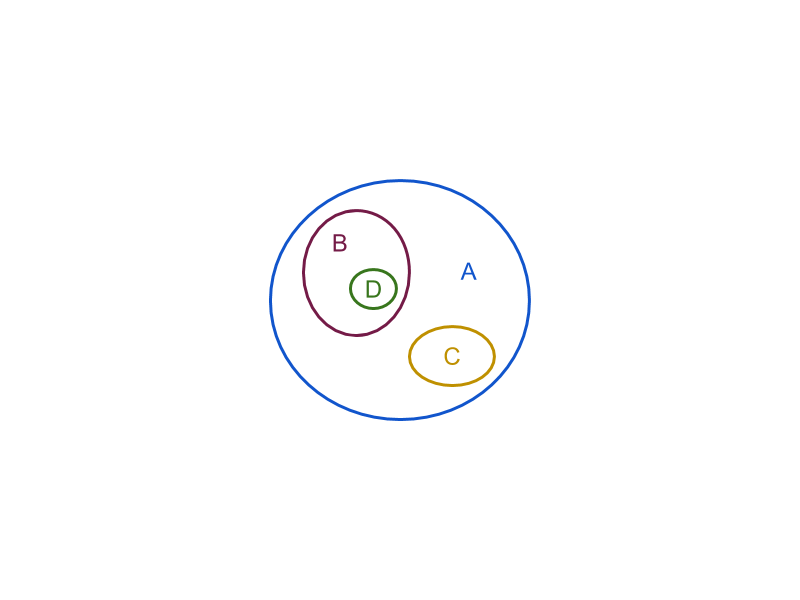
\includegraphics[width=\paperwidth]{../figs/nested_spheres.png}
 \caption{Nested spheres}
 \label{fig:spheres}
 \end{centering}
\end{figure}

There are a few fundamental assumptions made about the geometry file read in by this tool.  It is assumed 
that each surface meshset represents a closed surface, that there are no overlapping surfaces, and that there is a volume meshset that 
exactly corresponds to each surface meshset.  It is also assumed that the only hierarchical relationships that exist are the
parent-child relationships between volume and surface meshsets and that the surface 
meshset has forward sense with respect to its corresponding volume meshset.  The \texttt{Generate\_hierarchy} class
has two main public-facing functions \texttt{build\_hierarchy} and \texttt{construct\_topology} that can be used in sequence
to prepare a surface mesh geometry for MC radiation transport.  

\texttt{Build\_hierarchy} tests every surface in the geometry and decides where it belongs in a hierarchical tree.  
The hierarchical relationships will actually be made between volume meshsets which at this point, are the 
meshsets that exactly correspond to the surface meshsets.  The tree is formed by testing a point on the surface 
coming into the tree against the volumes already in the tree. Looking again at Figure~\ref{fig:spheres}, let’s assume that 
surface A is the first to be tested.  The tree is initially empty so volume A is automatically placed at the top.  
Assume surface C is tested next.  It is found to be inside of volume A, so it becomes a child.  Surface D is next 
and found to also be inside volume A, but neither inside or outside of volume C.  Volume D becomes another child of A.  
Last, surface B is tested.  It is found to be inside of A, outside of B, and beside C.  Therefore, volume B becomes a 
child of volume A, and a parent of volume D.  Because a volume can only have one parent, the parent-child linkage 
between volume A and volume D is broken.  The constructed tree is shown in Figure \ref{fig:tree} below.

\begin{figure}
 % Width = width of figure, {/path/to/figure.(png,pdf,jpg)}
 \begin{centering}
 \centering
 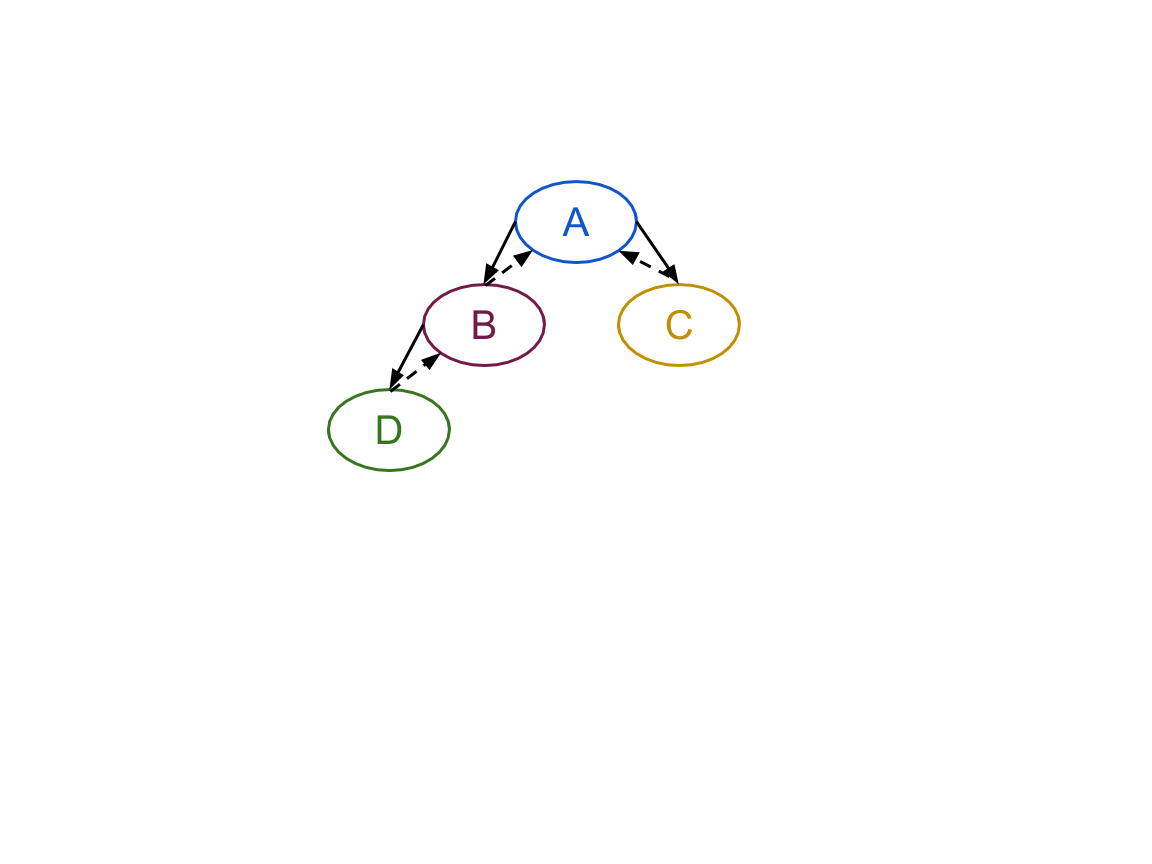
\includegraphics[width=\paperwidth]{../figs/tree.png}
 \caption{Hierarchical tree build from nested spheres geometry.}
 \label{fig:tree}
 \end{centering}
\end{figure}

After the hierarchical structure has been established, DAGMC-appropriate volumes are created by \texttt{construct\_topology}.  
This is accomplished by setting the surface sense and creating the hierarchical parent-child linkages between the 
surface meshsets.  Each surface has two volumes associated with it, one inside and one outside.  The surface has 
sense forward with respect to the volume it encloses and as mentioned earlier, this is already set. This function sets 
the reverse sense of the surface to the volume directly above it in the tree.  For example, surface B has forward 
sense with respect to volume B and reverse sense with respect to volume A.  Because surface A is the outermost surface, 
it has forward sense with respect to volume A and no reverse sense.  Surfaces that do not have reverse sense set lie in the 
implicit compliment.

% Combining Geometries
\subsection{Combining Geometries}
The \texttt{combine\_geoms} tool \cite{combine} was created for cases in which pieces of the full geometry are created
separately and then need to be combined together for the final radiation transport
calculation.  Each piece of the full geometry has its own set of meshsets that are usually assigned a global ID
that is an integer between 1 and n, where n is the total number of 
meshsets in that piece.  When several pieces of geometry are combined, the global ID of each
meshset needs to be reassigned a unique ID in order to avoid any overlap in ID space.  This tool loads each piece of
the geometry and then renumbers the global ID of every MOAB surface and volume meshset.


% SRAGCodes
\subsection{SRAGCodes}
The \texttt{SRAGCodes} repository is a software library that allows sampling of Galactic Cosmic Ray (GCR)
spectra for any Monte Carlo code. The library is written with C++ interfaces and coded using the C++11 
standard. The repository contains GCR spectra for Badhwar O'Neill 2014 Model (BOM), Local Interstellar Spectrum, and
the 1996 BOM model.

\subsubsection*{Build SRAGCodes}
To build the SRAGCodes repository, first clone the git repository from https://github.com/kerrylee01/SRAGCodes.git
\lstset{language=bash} 
\begin{lstlisting}
cd SRAGCodes
mkdir bld
cd bld
cmake .. -DCMAKE_INSTALL_PREFIX=..
make -j
make install
make test
\end{lstlisting}
The above listing shows the full install procedure including the running of the installation tests. In order to build
Fluka with the SRAGCodes linked in run the build\_fluka script found in the base directory of the SRAGCodes repository.
\subsubsection*{Running Fluka with SRAGCodes}
First, you must set the GCR\_SOURCE\_PATH environment variable to tell the Fluka executable where to find the GCR data. 
\begin{lstlisting}
export GCR_SOURCE_PATH=/path/to/SRAGCodes/RadSource/GCRSource/
\end{lstlisting}
In the Fluka input you wish to run you must add the source decription, there are currently two main types of 
geometric sampling, Spherical Element where you specify a target area and source radius and Sphere where an isotropic
inward directed. The geometry of the spherical element source is shown in Figure \ref{fig:spherical_element}.

\begin{figure}[ht!]
 \begin{centering}
 \centering
 \includegraphics[width=0.6\paperwidth]{../figs/spherical_element_source.png}
 \caption{Geometry of the input parameters for the Spherical Element source}
 \label{fig:spherical_element}
 \end{centering}
\end{figure}
Please note that the vertical shift is relative to the origin, so negative values mean the sphere origin is moved below the target plane
and positive values are above the source plane. Source particles are sampled by picking a random x,y coordinate in the range of the 
widths, a ray direction is istropically sampled in the positive z direction, and this ray is then intersected with the sampling sphere, 
this intersection point marks the start x,y,z coordinate of the source particle, the direction is similarly defined. The particle weight
is then set based on the solid angle of the target area from the intersection point, which effectively defines the probability of 
any source particle at this point intersecting with the target area. Please note that since particles are traced back from the target 
rectangle to the source sphere, particles are therefore sampled such that particles are born only above the visible horizon.  

\begin{table}[ht!]
 \begin{tabular}{c|c}
 Entry & Value \\
 \hline
 SDUM & SPHELE \\
 WHASOU(1) & X Origin (cm) \\
 WHASOU(2) & Y Origin (cm) \\
 WHASOU(3) & Z Origin (cm) \\
 WHASOU(4) & X Width  (cm) \\
 WHASOU(5) & Y Width  (cm) \\
 WHASOU(6) & Radius   (cm) \\
 WHASOU(7) & Z Shift  (cm) \\
 WHASOU(8) & Particle ID to sample \\
 WHASOU(9) & Source Type 
 \end{tabular}
\label{tab:sphele_source}
\caption{Source sampling options for the Spherical Element Source}
\end{table}

\begin{table}[ht!]
 \begin{tabular}{c|c}
 Entry & Value \\
 \hline
 SDUM & SPHERE \\
 WHASOU(1) & Radius (cm) \\
 WHASOU(8) & Particle ID to sample \\
 WHASOU(9) & Source Type 
 \end{tabular}
\label{tab:sphere_source}
\caption{Source sampling options for the Spherical source}
\end{table}

\subsubsection*{Particle ID}
Both of the source sampling methods require the entry of the particle id to sample,
\begin{table}[ht!]
 \begin{tabular}{c|c}
 Entry & Result \\
 \hline
 0  & sample all particles according to PDF \\
 1  & hydrogen isotopes only \\
 2  & helium isotopes only \\
 ... & ... \\
 28 & nickel isotopes only \\
 \end{tabular}
\label{tab:particleid}
\caption{Source sampling options for the Spherical source}
\end{table}

\subsubsection*{Source Type}
Both of the source sampling methods require the entry of the source type to sample
\begin{table}[ht!]
 \begin{tabular}{c|c}
 Entry & Result \\
 \hline
 0  & BOM Jan 2003 \\
 1  & BOM 2014 from 11/15/2015 to 1/15/2016 \\
 2  & BOM 2014 \\
 \end{tabular}
\label{tab:source_type}
\caption{Source sampling options for the Spherical source}
\end{table}

\subsubsection*{Source Sampling}
The main C++ layers of the SRAGCodes library is hideen behind a C safe callable routine that can be linked
against C/C++ and Fortran codes. The two functions exposed are \texttt{setup()} and \texttt{sample()}. 
\subsubsection*{setup}
The setup function is nessessarily long as we have to pass simple inputs to more complex C++ structures
in the SRAGCodes layer.
\lstset{language=C++}
\begin{lstlisting}
void setup_(double &origin_x, double &origin_y, double &origin_z,
        double &x_width, double &y_width, double &radius,
        double &z_shift, int &ionid, int &spectrum_type, int &error,
        char* src_type, int &string_length)
\end{lstlisting}

\subsubsection*{sample}
\begin{lstlisting}
void sample_source_(double *randoms, int& num_randoms, double &xxx, 
        double &yyy, double &zzz, double &uuu, 
        double &vvv, double &www, double &energy, 
        double &weight, double &atomic_mass,
        int &ionID, int &charge, int &nucleon_num)
\end{lstlisting}
There are two main ways of sampling from the source routine, either pass in a populated vector
of uniformly distributed random numbers e.g. \texttt{double array[6];} or 
\texttt{double precision array(6)} and set the \texttt{num\_randoms} variable to 6, or you 
can use the internal C++11 random number generator by passing an array and setting
\texttt{num\_randoms} to 1. The source routine will then return to you 
an appropriately distributed particle start coordinate \texttt{xxx},\texttt{yyy},\texttt{zzz} and
noramlised direction vectors \texttt{uuu},\texttt{vvv},\texttt{www}. The energy returned
in the \texttt{energy} variable is in GeV, the statistical weight \texttt{weight} is a weight
between 0 and 1. The ionId variable is Fluka specific and lets fluka know if it is a heavy
ion or not, in Fluka heavy ions are defined as particles with greater atomic number than 2. 
The atomic mass, charge and nucleon number serve to uniquely indentify the particle returned 
from the sampling routine. 



